%\section{Empirical Performance}
\label{sec:experiments}
% Experimental results

% Graphs
\begin{figure}[h]
\centering
\subfigure[$P_r$-Distributed Options]{
\includegraphics[height=2in]{figures/rooms-options}
\label{fig:rooms-options}
}
\subfigure[Return vs. Epochs]{
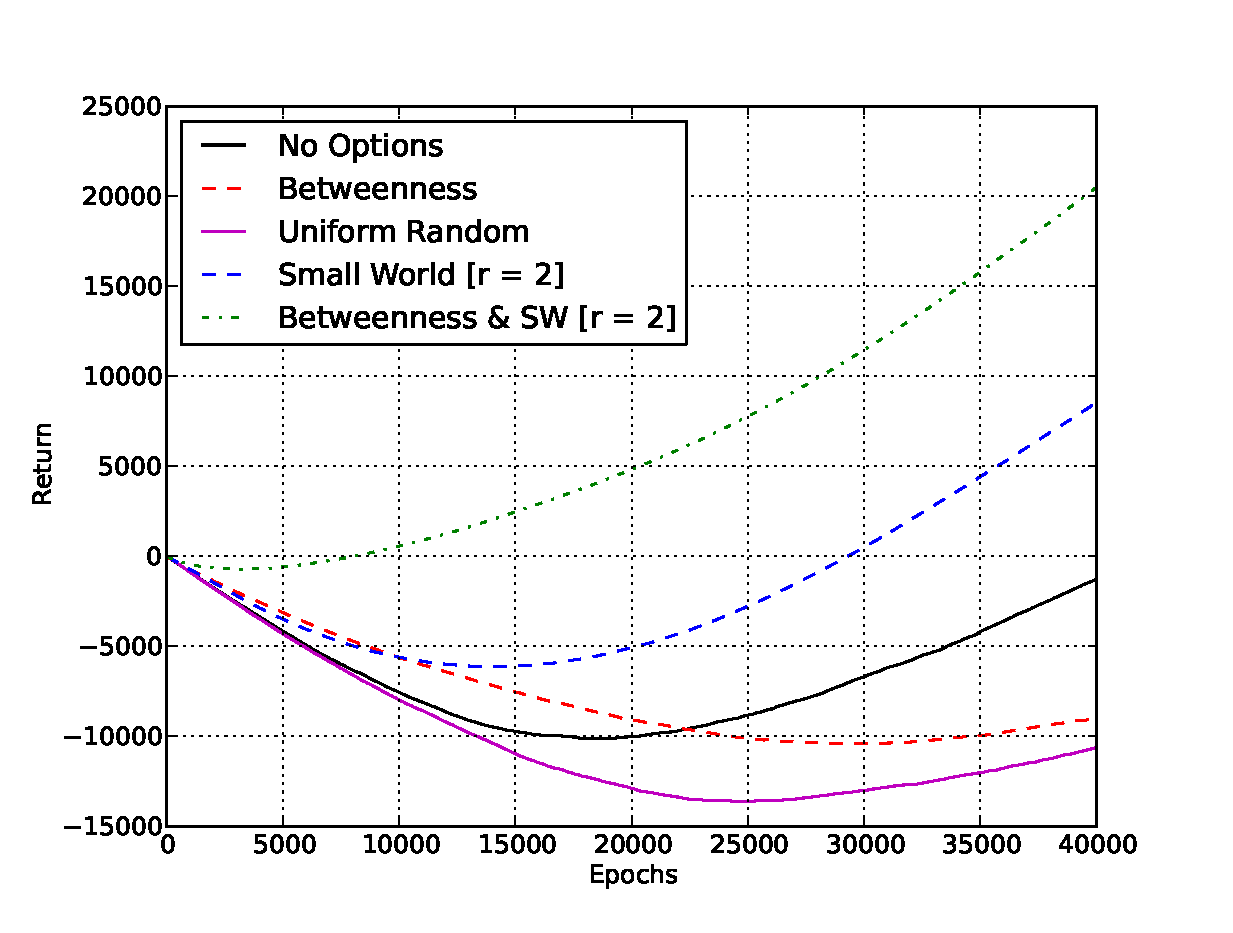
\includegraphics[height=2in]{figures/rooms-200-2}
\label{fig:rooms-performance}
}
\label{fig:rooms}
\caption{Results on the Rooms Domain}
\end{figure}

% Brief description of Rooms, Taxi and Arbitrary Navigation domains.
We trained agents using the MacroQ algorithm on three standard domains, Taxi,
Rooms and a $20\times20$ arbitrary navigation task. We compared the performance
of the agents using options generated (i) using betweenness centrality scores,
(ii) using paths between randomly selected nodes, (iii) using paths between
nodes selected using $P_r$, (iv) using a combination of (i) and (iii)
(Figure \autoref{fig:rooms}). While $P_r$-distributed options performed
well on the Taxi domain, they were not comparable to bottleneck-based methods,
as the goal state in this domain lies at a bottleneck state. In the Rooms and
Arbitrary Navigation domains however, we observed that $P_r$-distributed options
accumlated significantly more returns than other methods. 

% Observations
% When goal state and start state are further apart, the options that stand out
% are more

